% EnclosureDesignAndFabrication.tex
\subsection{Enclosure Design 3D print}  % to adapt from Nass here? no need to follow titles below, 
\label{subsec:enclosureDesign}
                                        % but keep \subsubsection{} to maintain structure
                                        % \chapter{Methodology} > \section{Prototype} > \subsection{Enclosure..}
This section provides an overview on the design and fabrication of the enclosure for the prototype. 
The enclosure is a critical component that houses the electronic components and provides protection against environmental factors. 
The design process involves several steps, including conceptualization, modeling, and fabrication.


\subsubsection{Conceptualization}
The design of the testing rig aperture underwent several iterations to optimize its performance and manufacturability. 
This iterative process approach allowed for the systematic refinement

\paragraph{Intial Concept Development}

An initial sketch design of the aperture consisted of a rectangle geometry “T-shaped” array of holes for the photodiodes to sit in with the main body being 105 mm long, 114 mm wide, and 1.5 mm gap in-between for a stripboard to be fitted in, these initial sketches can be seen in Appendix~\ref{app:AppendixE}.

\paragraph{CAD Software Selection and Workflow} 

Fusion 360 was employed for the CAD of the testing rig aperture, specifically for fabrication via 3D printing. 
Its capabilities in parametric modelling and integrated CAD/CAM workflows facilitated precise design execution and a streamlined transition to additive manufacturing, ensuring compliance with functional specifications. 
The software's simulation tools also enabled design optimisation for effective performance under testing conditions.

\subsubsection{Design Iterations and Refinements}
\paragraph{Intial Design}

For the initial design first made an outlined shape of the box with withe measurements of 115mm x 114mm and thickness of 1.5mm as can be seen in Figure~\ref{fig:CAD1}.
For the photo diode array used hole tool provided in fusion 360 and based the measurement values on the manufacturers datasheet for the photodiodes used for this project.



\begin{figure}[htbp]
    \centering
    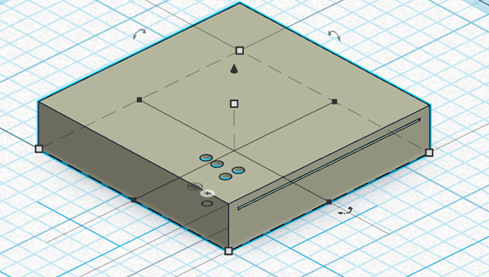
\includegraphics[width=0.7\textwidth]{figures/CAD-3DPrint/FirstIteration.png}
    \caption{First Design Iteration of the Enclosure}
    \label{fig:CAD1}
\end{figure}


\paragraph{Iteration 1}

Following the intial design sketches and CAD model, the first iteration of the enclosure was created as can be seen in Figure~\ref{fig:CAD2}.
The design focused on ensuring that the photodiodes were securely mounted and that the enclosure provided adequate protection for the electronic components. 
Iteration 1 involved a design refinement to facilitate modularity and interchangeability of photodiode array segments. 
Fusion 360's pattern tool was employed to replicate the photodiode hole arrangement across four distinct segments, ensuring consistent alignment and ease of component replacement.

\begin{figure}[htbp]
    \centering
    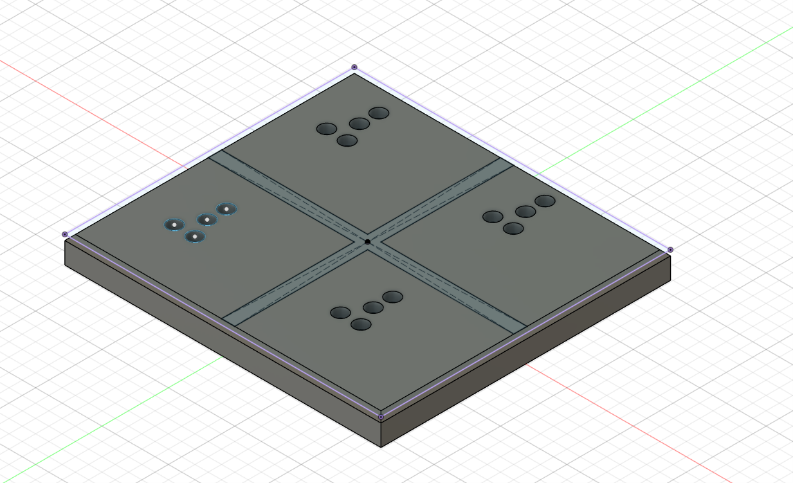
\includegraphics[width=0.7\textwidth]{figures/CAD-3DPrint/2ndIteration.png}
    \caption{Second Design Iteration of the Enclosure}
    \label{fig:CAD2}
\end{figure}

\paragraph{Iteration 2}

In iteration 2 reduced iteration 1's size down to one of the segments which measured out at 52mm length, 57mm and 10mm height with the focus being the housing for the photodiode array, shown in Figure~\ref{fig:CAD3}

\begin{figure}[htbp]
    \centering
    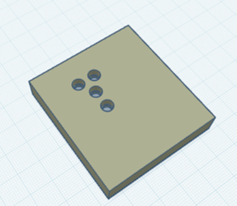
\includegraphics[width=0.7\textwidth]{figures/CAD-3DPrint/3rdIteration.png}
    \caption{Third Design Iteration of the Enclosure}
    \label{fig:CAD3}
\end{figure}

\paragraph{Refinements}

To address dimensional incompatibility from previous iterations, the CAD model was revised. 
In iteration 3, the extruded height was increased by [insert height dimension] to achieve a proper fit. 
This adjustment was made while maintain the ease of fabrication and assembly.
The final aperture design as depicted in Figure~\ref{fig:CADFinal} while also utilizing a rail system such as a T rail to allow, incorporates the necessary dimensional adjustments and structural refinements identified through the print-and-test iterations. 
This design ensures proper mounting and functionality within the testing rig. 
With the final, validated design, the CAD model was prepared for the final 3D printing fabrication, ensuring optimal orientation to accurately replicate the refined dimensions.

\begin{figure}[htbp]
    \centering
    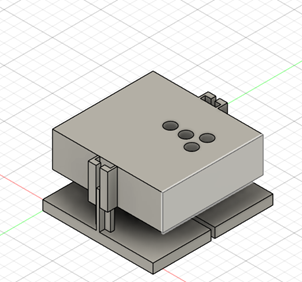
\includegraphics[width=0.7\textwidth]{figures/CAD-3DPrint/FinalCAD.png}
    \caption{Final Design Iteration of the Enclosure}
    \label{fig:CADFinal}
\end{figure}

\subsubsection{Parametric Deesign Considerations}
The initial design measured 105 mm long, 114 mm wide, and 20mm depth and 1.5 mm gap. 
Subsequent work resulted in revisions, with the second redesign extending the dimensions to 150 mm in length, 115 mm in breadth, and 10 mm in thickness for testing. 
The final design was improved to be 52 mm long, 57 mm wide, and 10 mm height with a rail system added for adjustable height. 
These improvements were made to improve the design for stability.

\subsubsection{Overview of 3D Printing methods}

\paragraph{Fused Deposition Modelling (FDM)}

Fused deposition modelling is a popular Additive manufacturing (AM) Method because of its fast production, cost efficiency, and ease of access. 
Broad material adaptation and capability to produce complex components \cite{RefWorks:RefID:89-rajan2022fused}. 
It works by using a material extrusion process, where a continuous filament of thermoplastic or composite material is used to construct 3D parts. 
The polymer filament is forced over the nozzle and fed over the build plate or preciously solidified substance, and the product is built through a layer-by-layer method while maintaining a steady speed and pressure \cite{RefWorks:RefID:86-lee2017fundamentals}. 

\paragraph{Stereolithography (SLA)}

Stereolithography is a 3D printing technology that uses liquid photopolymer that polymerises when exposed to a laser. 
The worktable moves up and down after being immersed in resin.  
The photopolymer hardens after being selectively irradiated with a laser beam. 
The printed object becomes a detailed physical model from the bottom up \cite{RefWorks:RefID:63-yankov2017comparison}.

\begin{figure}[htbp]
    \centering
    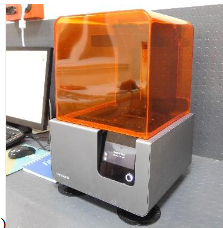
\includegraphics[width=0.7\textwidth]{figures/CAD-3DPrint/SLAPrinter.png}
    \caption{SLA Printer}
    \label{fig:SLA}
\end{figure}

\paragraph{Selective Laser Sintering (SLS)}
Carl Deckard developed selective laser sintering (SLS) in 1987, and it is among the best powder-based AM methods \cite{tiwari2015selection}. 
The solid structure is created in this method by sintered powder particles using a laser source \cite{RefWorks:geng2019mechanical}. 
This SLS process uses two chambers: the building chamber is used for printing, and the feed chamber loads the powder onto the bed using a roller. 
First, a roller in the feed chamber distributes the powder evenly onto the constructed chamber base plate. 
The building chamber is heated to a temperature below melting point before the carbon dioxide (CO2) laser is shone on the powder to cure it. 
Next, the building chamber descends a little, and the feed chamber applies the powder over the printed layers. 
After construction is finished, the extra powders that served as a supporting framework in the building chamber are removed, and the extra material is recycled. 
This process for creating high-density prototype goods is flexible and economical \cite{RefWorks:niu2018review}. 
However, compared to the SLS method, the operation cost is expensive, and the product quality is bad because of the high power of the laser input \cite{RefWorks:RefID:84-de2016high}.

\subsubsection{Justification for FDM printing}
For this project, FDM was decided as the main manufacturing method for our CAD design this is due to benefits such as: 

\paragraph{Accessibility and Affordability}

In addition to its low cost and ease of use, FDM's ability to produce complicated geometries reinforces its standing as the leading option for small-scale prototyping. 
The capacity to create elaborate designs with different layer heights can greatly improve the precision of microscopic features, which is critical in applications like microfluidics and biomedical devices \cite{RefWorks:RefID:61-ameen2024exploring}. 
SLA may provide better surface smoothness and precision, but it is more expensive and requires more post-processing, making it less accessible for rapid prototyping \cite{RefWorks:altuğ2022comparison}. 
While SLA and SLS are valuable alternatives, FDM's capabilities make it an indispensable tool for designers and engineers looking for fast and cost-effective solutions in their projects.

\paragraph{Post-processing Requirements}

Furthermore, the environmental impact of 3D printing processes is becoming a more essential factor for designers and engineers. 
While FDM uses recyclable thermoplastic materials, other techniques, such as SLA, frequently rely on resins, which may offer disposal issues due to their chemical makeup \cite{RefWorks:yankov2017comparison}. 
As the industry progresses towards more sustainable practices, optimising material selection not only lowers costs but also reduces environmental footprints, making FDM a more appealing alternative in this aspect. 
Furthermore, developments in biodegradable filaments are increasing FDM's attractiveness, allowing for prototypes that line with eco-friendly goals while maintaining performance and quality. 
Thus, FDM's mix of cost, adaptability, and low environmental effect places it at the forefront of the growing additive manufacturing industry.

\subsubsection{Material Selection}
\paragraph{Overview of Material Properties}
The material properties of 3D printed parts are critical for their performance in various applications, for FDM printing, there are various filament materials such as acrylonitrile butadiene styrene (ABS), Polylactic acid (PLA), Polyetheretherketone (PEEK), polypropylene (PP), and Thermoplastic Polyurethane (TPU) \cite{RefWorks:RefID:89-rajan2022fused}.

\paragraph{Cost Considerations}

When selecting materials for 3d printing, cost is a significant factor. 
PLA is one of the most cost-effective option available as its one of the more widely used filaments in FDM due to its thermal and rheological properties \cite{RefWorks:RefID:89-rajan2022fused}, which make it easier to manufacture parts.

\subsubsection{3D Printer Selection and Specifications}
The Creality Ender 3 SE(Figure~\ref{fig:NassPrint}) was selected as the Fused Deposition Modelling (FDM) printer for this project due to its efficiency and reliability. 
Its single-extrusion design, coupled with an automated Z-offset levelling system, significantly reduces recalibration requirements, ensuring consistent print quality and minimising downtime. 

\begin{figure}[htbp]
    \centering
    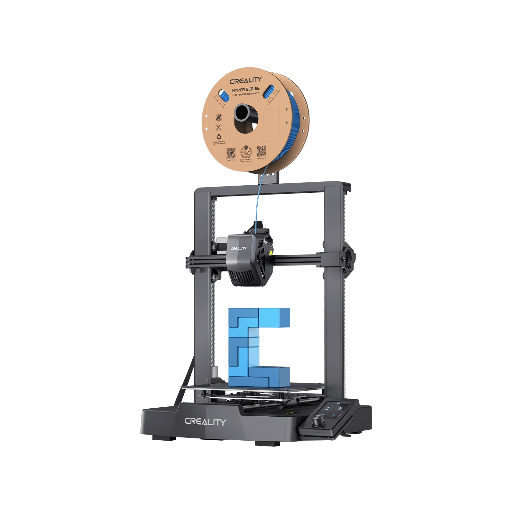
\includegraphics[width=0.7\textwidth]{figures/CAD-3DPrint/NassPrinter.png}
    \caption{Creality Ender V3 SE}
    \label{fig:NassPrint}
\end{figure}

The layout of the FDM process is shown in Fig. Here the filament is stored in the spool roller and is connected directly to the extrusion head i.e. extrusion head. 
This head will move in X and Z-directions while the build plate will move in the Y-direction. 
Electric motors will control the position of the moveable liquefier \cite{RefWorks:RefID:85-mohd2020review}. 
Generally, for this process material filaments are used for both the supporting and built material of the print.

\begin{figure}[htbp]
    \centering
    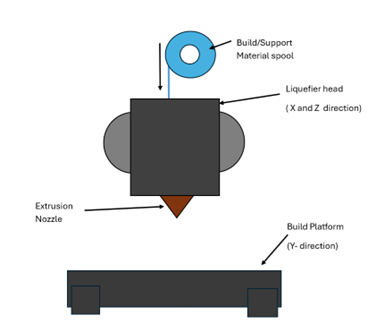
\includegraphics[width=0.7\textwidth]{figures/CAD-3DPrint/FDMProcess.png}
    \caption{Single Head FDM Process Layout}
    \label{fig:FDMProcess}
    
\end{figure}

This FDM technique generally consist of three sections being the pre-processing, production and post processing. 
In the pre-processing stage the product is created using CAD Software and saved in STL format. 
Before slicing the file, key parameters such as slicing settings, build orientation and machine temperature are considered. 
These crucial parameters Influence the final products mechanical properties. Figure~\ref{fig:FDMparameters} shows the necessary process parameters. 
After this step, slicing is performed using the Software Ultimaker Cura and the tool path is generated as G-code which is a computer numerical control code used to manage the extrusion process.

\begin{figure}[htbp]
    \centering
    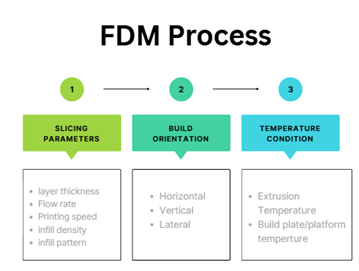
\includegraphics[width=0.7\textwidth]{figures/CAD-3DPrint/FDMflowchart.png}
    \caption{FDM Parameters }
    \label{fig:FDMparameters}
    
\end{figure}

\begin{figure}[htbp]
    \centering
    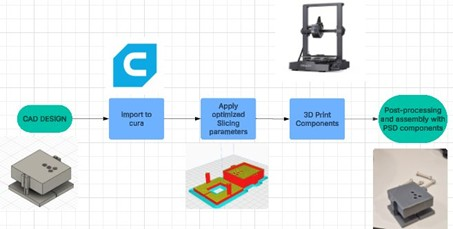
\includegraphics[width=0.7\textwidth]{figures/CAD-3DPrint/FullFlowChart.jpg}
    \caption{Flowchart of the FDM Process}
    \label{fig:FDMflowchart}
    
\end{figure}

\subsubsection{Print Settings and Parameters} 
\paragraph{Infill Pattern}

The infill pattern offers internal support to the 3D print as it develops each layer. 
Printing layers without an infill pattern would be time-consuming and result in material slumping over empty areas \cite{RefWorks:RefID:88-srinivasan2020impact}. 
The figure below displays several infill patterns, including triangular, grid, cubic, honeycomb, concentric, rectilinear, rectangular, octet, and wiggly. 
For this project, the cubic infill pattern was selected due to its advantages that align with our project's requirements. 
Firstly, the cubic pattern provides reliable mechanical properties ensuring robust structural support and strength, which is necessary for the housing component of the design. 
Secondly, the cubic infill pattern is efficient in terms of print speed. 
It allows for faster printing compared to other infill patterns without compromising its structural efficiency. 
These benefits make the cubic infill pattern an ideal choice for achieving the desired balance between strength and efficiency in the printed parts

\begin{figure}[htbp]
    \centering
    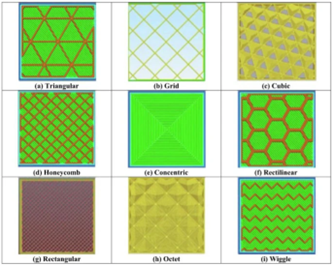
\includegraphics[width=0.7\textwidth]{figures/CAD-3DPrint/infillPatterns.png}
    \caption{Various Infill Patterns Used for FDM Processes}
    \label{fig:infillpatterns}
    
\end{figure}

\paragraph{Infill Density}

Mechanical performance of 3D-printed components is largely determined by the infill density, which dictates the amount of material used internally \cite{RefWorks:RefID:89-rajan2022fused}.
Groza and Shackelford \cite{srivatsan2012materials} categorise infill patterns into three distinct types, each impacting the mechanical properties and print efficiency of 3D-printed components. 
The `solid normal' infill, characterised by its dense interior, yields robust mechanical performance. 
Conversely, the `sparse' infill pattern prioritises reduced printing time and material consumption by incorporating gaps and utilising a unidirectional raster. 
The `sparse double dense' infill, while also focusing on minimising printing time and material usage, employs a crosshatch raster pattern. 
However, for the fabrication of the testing rig aperture in this project, a 15\% infill density was employed, which lies within the sparse categorisation, to achieve a balance between structural integrity and material efficiency.

 \paragraph{Printing Speed}

 Printing speed is the nozzle's pass-through speediness on the build platform when printing. 
 The printing speed determines how long the product takes to produce. 
 In addition, the printing speed has a maximum effect on the deformation of the product since, during production, this quick printing could produce significant residual stresses\cite{RefWorks:RefID:89-rajan2022fused}. 
 For this project a nozzle speed of 180 mm/s was chosen, as it showed the best performance than other nozzle speeds when doing test calibrations. 

\paragraph{Operating Temperature}

Rajan et al. (2022) emphasise the vital role of operating temperatures in 3D printing, particularly nozzle temperature (extrusion temperature) and bed temperature (build platform temperature). 
Prior to printing, the nozzle is heated to a temperature sufficient to melt the filament, allowing extrusion. 
Simultaneously, the build platform is heated to a bed temperature that promotes good adhesion and reduces warping during printing \cite{RefWorks:RefID:89-rajan2022fused}.

\paragraph{Nozzle Temperature}

The choice of 200°C for PLA extrusion was determined through a combination of filament manufacturer guidelines and experimental optimisation. 
This temperature facilitated adequate melt flow, enabling proper layer bonding and minimising the risk of under-extrusion. 
Lower temperatures resulted in insufficient melt flow, leading to weak layer adhesion, while higher temperatures increased the potential for stringing and warping. 
Therefore, 200°C was identified as the optimal setting to achieve consistent and reliable print quality for the testing rig aperture.

\paragraph{Build Orientation}

To optimise the dimensional accuracy of the photodiode hole array and minimise the need for extensive support structures, the testing rig aperture was printed in a horizontal orientation. 
This orientation, as shown in Figure, placed the top surface, containing the critical photodiode holes, directly on the build plate. 
This reduced the potential for surface imperfections caused by support structures on these critical features and facilitated a more uniform thermal distribution during printing.

\begin{figure}[htbp]
    \centering
    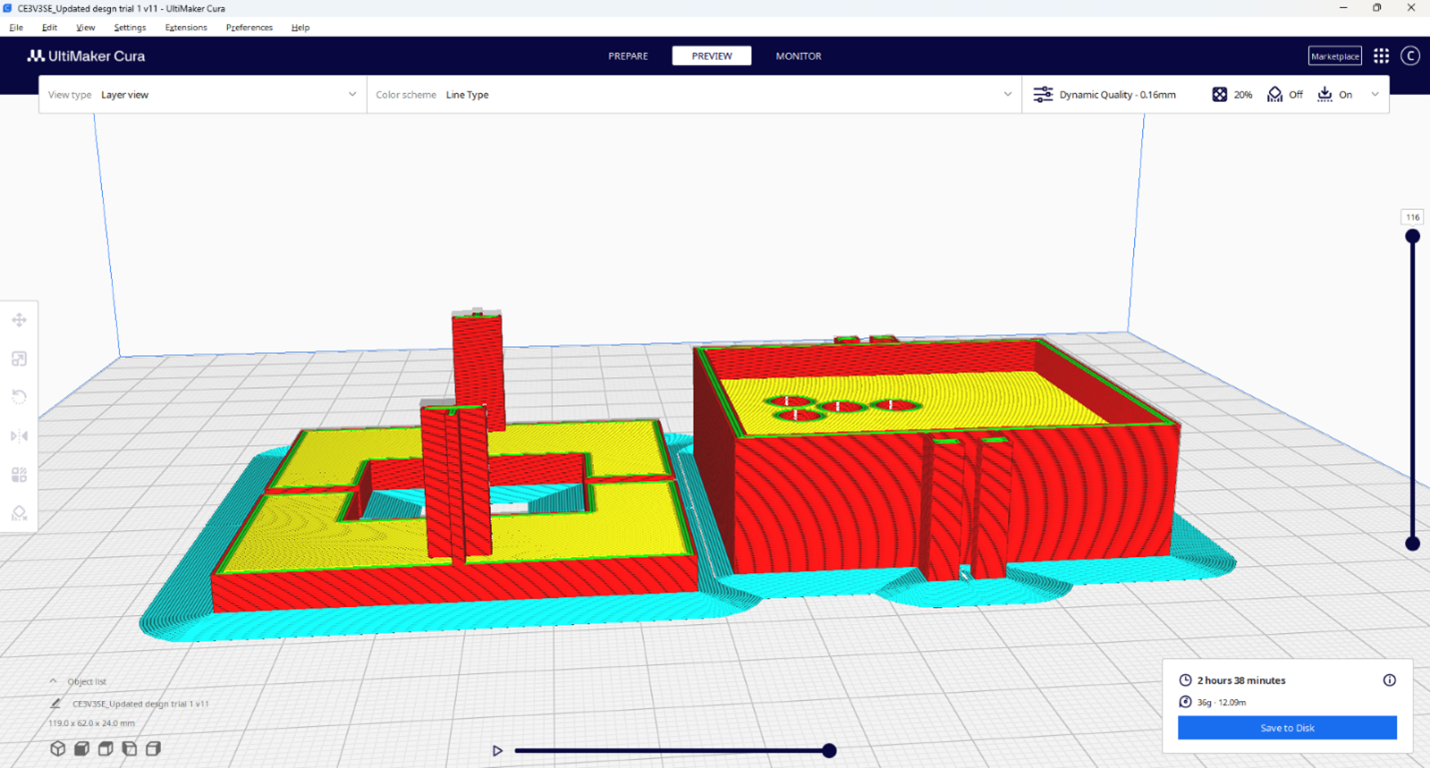
\includegraphics[width=0.7\textwidth]{figures/CAD-3DPrint/SLICED.png}
    \caption{Design Sliced for Printing}
    \label{fig:sliced}
   
    
\end{figure}

\subsubsection{Iterations and Improvements}
There were two main challenges that we came across during the printing process, which were bed adhesion and dimensional inaccuracy.

\paragraph{Bed Adhesion}

For the bed adhesion issue shown in Figure~\ref{fig:Fail1}, we found that the source of the issue was temperature related. 
Firstly, the build plate temperature was 45$^{\circ}$C which was lower than that what is recommended when printing with PLA which ranges from 50$^{\circ}$C - 70$^{\circ}$C. 
Additionally the extrusion temperature was 190$^{\circ}$C which is on the lower end of the recommended range which is typically 190$^{\circ}$C - 220$^{\circ}$C \cite{RefWorks:RefID:91-unionfab2025ultimate} after some testing to find the ideal which was found to be at 60$^{\circ}$C.
So, after some readjustments to the build plate and extrusion temperature, a first layer was able to stick to the build plate without any warping happening shown in Figure~\ref{fig:Fail2}.
Although the first layer print worked, there was still warping on the corners of the prints, as well as some 'wisping' on the surface, so research was conducted to find a solution, which was to use a brim on the print shown \ref{fig:Brim}.
This is an extra layer of material printed around the base of the print object. 
This increased the surface area contact with the build plate, improving adhesion and stability during printing. 
These methods significantly reduced bed adhesion issues, leading to more successful and reliable prints as can be seen in Figure~\ref{fig:BedAdImproved}

\begin{figure}[htbp]
    \centering
    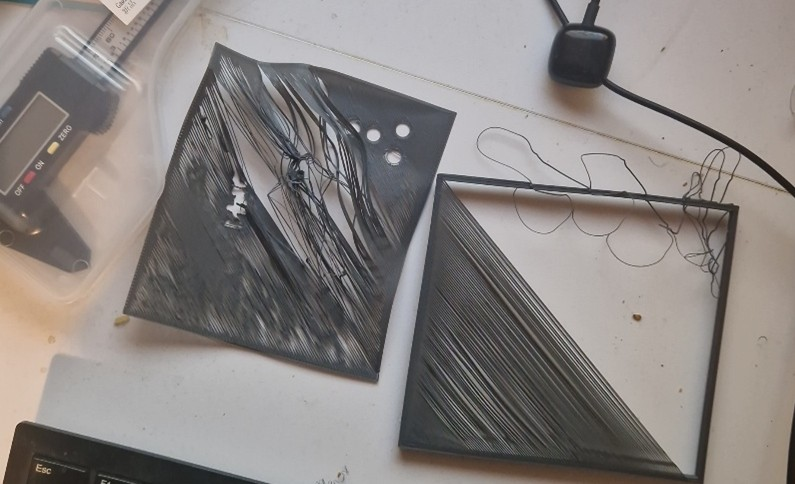
\includegraphics[width=0.7\textwidth]{figures/CAD-3DPrint/FAIL1.jpg}
    \caption{Bed Adhesion Failure}
    \label{fig:Fail1}
   
    
\end{figure}

\begin{figure}[htbp]
    \centering
    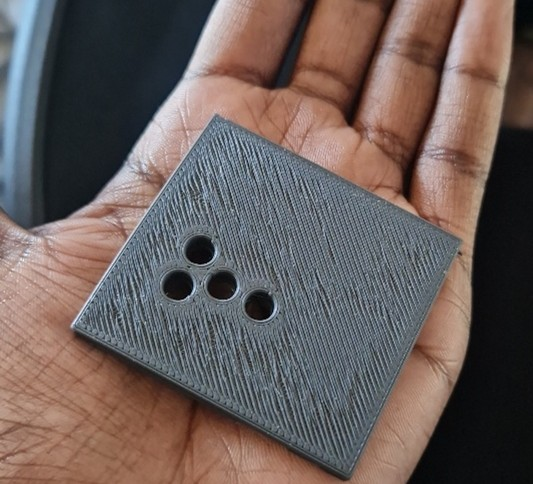
\includegraphics[width=0.7\textwidth]{figures/CAD-3DPrint/FAIL2.jpg}
    \caption{Test Print After Temperature Adjustments}
    \label{fig:Fail2}
   
    
\end{figure}

\begin{figure}[htbp]
    \centering
    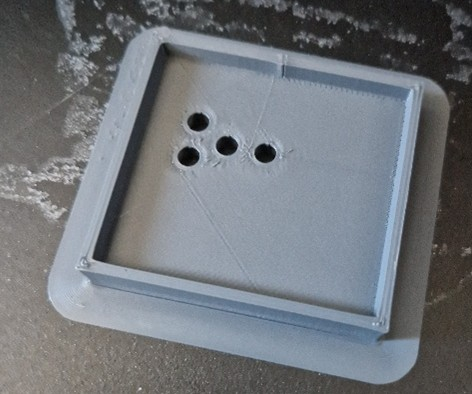
\includegraphics[width=0.7\textwidth]{figures/CAD-3DPrint/CADwitDaBrim.jpg}
    \caption{Part Printed with Brim}
    \label{fig:Brim}
   
    
\end{figure}

\begin{figure}[htbp]
    \centering
    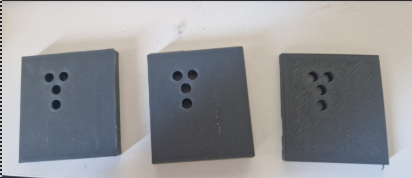
\includegraphics[width=0.7\textwidth]{figures/CAD-3DPrint/BedAdImproved.png}
    \caption{Improved Bed Adhesion from Test Print Attempts}
    \label{fig:BedAdImproved}
   
    
\end{figure}

\paragraph{Dimensional Inaccuracy}

Another one of the issues encountered in this project was the dimensional inaccuracies specifically the hole sizes for the test rig in which the CAD model did not translate entirely to the 3D printed part.  
After doing some fault finding it was found that over time as the printing process continued some of the printed layers had begun to cool, thus shrinking down the holes made for the photodiode array, causing them to not fit as can be seen in Figure~\ref{fig:DimInaccuracy}.  
To address dimensional inaccuracies between printed apertures and electronic components, an iterative calibration process was conducted using Ultimaker Cura's hole expansion feature. 
This technique, which involves adjusting the horizontal dimensions of the print, is essential for several reasons. 
Primarily, it compensates for material shrinkage, a common occurrence during FDM printing, ensuring dimensional accuracy. 
Furthermore, by fine-tuning the dimensions of slots and holes, it facilitates improved fit and alignment of components like photodiodes. 
Ultimately, this adjustment enhances the precision of the printed part, ensuring that critical components are placed accurately, thereby preserving the design's intended functionality. 
Through this process, an expansion of 0.16mm was determined to be optimal, ensuring precise integration of electronic components.

\begin{figure}[H]
    \centering
    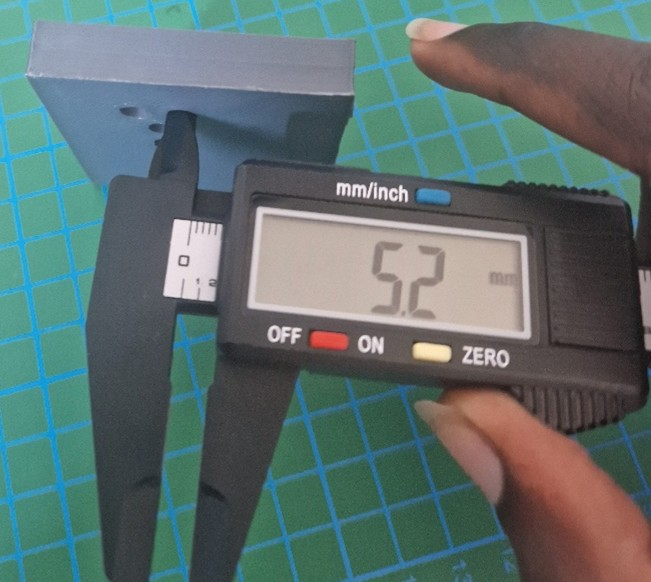
\includegraphics[width=0.7\textwidth]{figures/CAD-3DPrint/WrongDimensions.jpg}
    \caption{Dimensional Inaccuracy of the Holes after Printing}
    \label{fig:DimInaccuracy}
    
   
    
\end{figure}
%
% templates for figures, code, 
%

% %%% display code nicely
% \begin{lstlisting}[style=cstyle, caption=System Architecture Code Example, label=lst:SystemArchitecture7]
% # Your code here
% \end{lstlisting}

% \begin{figure}[htbp] %h-ere t-op b-ottom p-page (separte) -good to allow all htbp to give the compiler more options
%     \centering
%     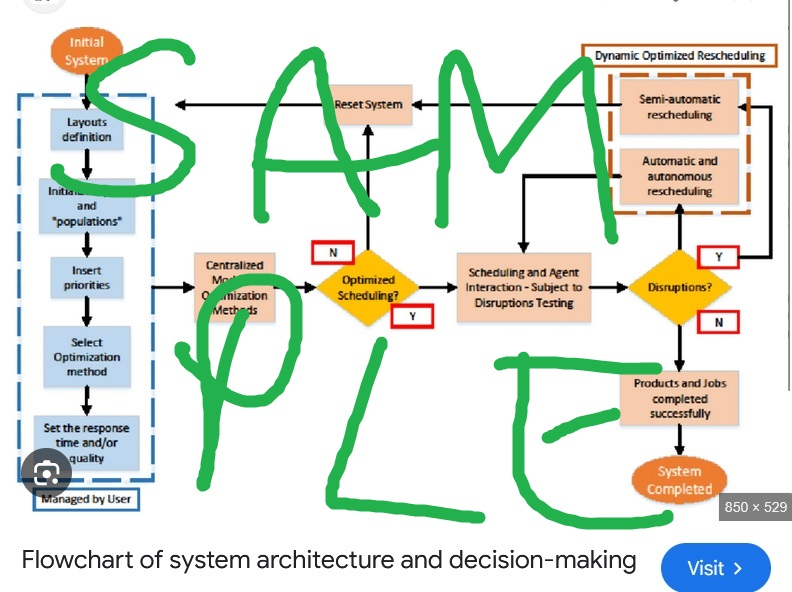
\includegraphics[width=0.6\textwidth]{figures/methodology/system_architecture.jpg}
%     \caption{System Architecture Diagram}
%     \label{fig:system-architecture2}
% \end{figure}

% % Include a flowchart in LATEX format
% \begin{figure}[H]
%     \centering
%     \scalebox{0.8}{ % Scale to 80% of original size
%         % try generating flowcharts as svg in Claude 
% and edit with inkscape instead of this.
% but claude did generate this one so might 
% be useful too but you can't easily make
% small repairs in inkscape


% CNN Transfer Learning Flowchart - Compact Multi-Column Layout
% \begin{figure}[htbp]

\centering
\resizebox{\textwidth}{!}{ % Scale to fit width while maintaining aspect ratio
\begin{tikzpicture}[node distance=0.8cm and 1.5cm, auto]
    % Define a smaller block style
    \tikzset{
      block/.style = {rectangle, draw, fill=blue!20, 
                      text width=7em, text centered, rounded corners, minimum height=1.8em, font=\small},
    }
    
    % Brazilian model training - Column 1
    \node [block] (brazildata) {Download Brazilian coins dataset};
    \node [block, below=of brazildata] (extract) {Extract dataset};
    \node [block, below=of extract] (setup) {Setup directories};
    \node [block, below=of setup] (define) {Define train/val dirs};
    \node [block, below=of define] (create) {Create CNN architecture};
    \node [block, below=of create] (compile) {Compile the CNN};
    \node [block, below=of compile] (train) {Train model};
    \node [block, below=of train] (trained) {Model trained (5 classes)};
    
    % Transfer learning - Column 2 (Middle)
    \node [block, right=2.5cm of brazildata] (freeze) {Freeze all layers};
    \node [block, below=of freeze] (replace) {Replace final layers};
    \node [block, below=of replace] (add) {Add regularization and dropout};
    \node [block, below=of add] (output) {New output layer (8 classes)};
    \node [block, below=of output] (finaltrain) {Train and fine-tune};
    \node [block, below=of finaltrain] (inference) {Perform inference on new coins};
    
    % UK data preparation - Column 3 (Right)
    \node [block, right=2.5cm of freeze] (ukdata) {Download UK coins dataset};
    \node [block, below=of ukdata] (ukextract) {Extract UK dataset};
    \node [block, below=of ukextract] (uksetup) {Setup UK directories};
    \node [block, below=of uksetup] (ukgen) {Create data generators (80/20 split)};
    
    % Connect all nodes with arrows
    \path [line] (brazildata) -- (extract);
    \path [line] (extract) -- (setup);
    \path [line] (setup) -- (define);
    \path [line] (define) -- (create);
    \path [line] (create) -- (compile);
    \path [line] (compile) -- (train);
    \path [line] (train) -- (trained);
    
    \path [line] (ukdata) -- (ukextract);
    \path [line] (ukextract) -- (uksetup);
    \path [line] (uksetup) -- (ukgen);
    
    % Connect the columns
    \path [line] (trained) -- node[midway, above] {Transfer} (freeze);
    \path [line] (ukgen) |- (finaltrain);
    
    % Connect middle column
    \path [line] (freeze) -- (replace);
    \path [line] (replace) -- (add);
    \path [line] (add) -- (output);
    \path [line] (output) -- (finaltrain);
    \path [line] (finaltrain) -- (inference);
    
    % Group boxes to show different stages with smaller padding
    \begin{pgfonlayer}{background}
        \node[group={[yshift=0.3cm]above:Brazilian Model Training}, fit={(brazildata) (extract) (setup) (define) (create) (compile) (train) (trained)}, inner sep=0.2cm] {};
        \node[group={[yshift=0.3cm]above:UK Data Preparation}, fit={(ukdata) (ukextract) (uksetup) (ukgen)}, inner sep=0.2cm] {};
        \node[group={[yshift=0.3cm]above:Transfer Learning}, fit={(freeze) (replace) (add) (output) (finaltrain) (inference)}, inner sep=0.2cm] {};
    \end{pgfonlayer}
\end{tikzpicture}
}
% \caption{CNN Transfer Learning Flowchart: Brazilian to UK Coins}
% \label{fig:cnn-flowchart}
% \end{figure}
%     }
%     \caption{System Design Overview Flowchart}
%     \label{fig:decriptiveLabel11} % descriptive to call in text with \ref{fig:decriptiveLabel}
% \end{figure}